\section{Analýza stavu}
\subsection{Operačné systémy}
\indent Informatika a informačné technológie je pomerne mladá vedná disciplína. Jej začiatky je možné datovať od druhej polky dvadsiateho storočia, čo momentalne predstavuje necelých sedemdesiat rokov. Za tento čas informatika zaznamenala enormný rast či vo vývoji hardwéru alebo softwéru.  Operačný systém je základná časť akéhokoľvek počítaťového sytému, je to kus softvéru, ktorý umožnuje počítačom fungovať. Oblasť operačných systémov v poslednej dobe prechádza rapídnymi zmenami nakoľko počítače sa stali súčasťou každodenného života od malých zariadení napríklad v automobiloch až po najsofisitkovanejšie servery nadnárodných spoločností. Aj keď v dnešnej dobe poznáme mnohé operačné systémi, my sa zameriame na Windows, Mac OS, Unix a Linux.\cite{osbook}
% tuto cast este asi rozsirim 
\subsubsection{Windows}
\indent Microsoft Windows uviedol svoje prvé operačné systémy v roku 1985 ako nadstavbu MS DOS. Jeho popularita rýchlo rástla až vyvrcholila dominantným postavením na trhu v osobných počítačoch. V roku 1993 začal vydávať špecializované operačné systémy pre servery, ktoré prinášali novú funkcionalitu pre počítače používané ako servery. Pre účely automatizácie sa na Windows serveroch používajú hlavne powershell scripty, písane v rovnomennom jazyku powershell.
\paragraph{Predinštalovaný software}
\indent Málo predinštalovaného softvéru jedine powershell na widows serveri je defaultne, ostatné programátorské tooly je potrebné stiahnúť dodatočne. 
\newline
\subsubsection{MacOs}
\indent  Mac tiež ponúka serverovú verziu svojho operačného systému pod názvom OS X Server, ktorý začal písať svoju históriu v roku 2001, avšak neteší sa takej obľube ako Windows, unix alebo linux server. Skriptovacím jazykom pre OS X server nieje špecifický jazyk, je možné vybrať si z Pythonu, JavaSriptu, Perl, AppleScriptu, Swiftu alebo napríklad Ruby. Každý jazyk prináša určité plusy, ale zároven mínusy čo je však najpodstatnejšie nie je tam štandardizovaný skriptovací jazyk.
\paragraph{Predinštalovaný software}
\indent Predinštalovaný software pre developerov na Mac OS je python, apple script, Ruby, bash, objective-c. Donedávna bola štandardom aj Java.

\subsubsection{Unix}
\indent Patrí medzi prvé operačné systémy pre servery, ktorých vývoj začal v roku 1970 v priebehu rokov vzniklo nespočetné množstvo nových verzií Unixu. Unixové servery sa tešil veľkej obľube hlavne v minulosti momentálne sú na ústupe hlavne kvoli vyšším nákladom na ich zaobstaranie a prevázku. Pre účely unixu sa vytvoril Unix shell, oľúbený scriptovací jazyk, ktorý sa v rôznych obmenách teší veľkej obľube medzi administrátormi a automatizačnými programátormi.
\paragraph{Predinštalovaný software}
\indent Na vačšine unixových systémoch je predinštalovaný bash a open JDK.
\newline
\subsubsection{Linux}
\indent  Prvé vydanie Linux  bolo 17. septembra 1991, bol rozšírený na najviac platforiem a momentálne sa pýši tým, že je jediný používany operačný systém na TOP 500 superpočítačoch(mainframoch) Skriptovací jazyk Unix shell resp. jeho najrozšírenejšia forma Bash.
\paragraph{Predinštalovaný software}
\indent Predinštalovaný software vo väčšine distribúciách linuxu sú bash, Open Jdk - Java, niektoré distribúcie ponúkajú Python. RedHat začína s podporou .net frameworku.
\newline
\subsection{Programovacie jazyky}
\indent S príchodom osobných počítačov no najmä serverov, sa programátori zaujímali o automatizáciu procesov, ktoré na danom stoji bolo spočiatku potrebné spúšťať manuálne. Nakoľko tieto úlohy neboli na toľko komplexné ako samotné programy, ktoré spúštali bolo vhodné na tieto úlohy využiť/vytvoriť skriptovacie jazyky. V nasledujúcej časti si priblížime zopár programovacích jazykov, ktoré sa v dnešnej dobe bežne používajú na tvorbu automatizovaných skriptov.

\subsubsection{Shell}
\indent
Je skriptovacím jazykom pre unixové distribúcie. Počas rokov prešiel roznymi zmenami a rozšíreniami. Verzie shellu su: sh, csh, ksh,tcsh, bash. Bash sa momentálne teši najväčšej obľube no zsh je verzia shellu, ktorá má najviac rôznych rozšírení funkcionality ako aj veľa priaznivcov medzi developermi. V nasledujúcich častiach všeobecne zhodnotíme jednotlivé výhody resp. nevýhody tohoto skriptovacieho jazyka.

\paragraph{Výhody}
\begin{itemize}
	\item automatizácia často opakujúcich sa úloh
	\item dokáže zbiehať zloťité zloťené príkazy ako jednoriadkový príkaz  - tzv. reťazenie príkazov
	\item ľahký na používanie
	\item výborné manuálové stránky
	\item ak hovoríme o Unix shelli je portabilný naprieč platformami linuxu-unixu
	\item jednoduché plánovanie automatických úloh
	\newline
\end{itemize}
\paragraph{Nevýhody}
\begin{itemize}
	\item asi najväčšou nevýhodou je ze natívne nefunguje pod windowsom, existuju iba rozne emulátory a nástroje tretích strán, ktoré sprostredkujú jeho funkcionalitu.
	\item pomalé vykonávanie príkazov pri porovnaní s inými programovacími jazykmi
	\item nový proces pre skoro každý spustený príkaz
	\item zložitejší na pamatanie si rôznych prepínačov, ktoré dané príkazy podporujú
	\item nejednotnosť prepínočov(hoc to by asi ani nešlo)
	\item neprenosný medzi platformami
	\item shell nepridáva vlastné príkazy, používa iba tie, ktoré sú dostupné na konkrétnom počítači
\end{itemize}
\paragraph{Popis a zhodnotenie jazyka}
\indent
Unix Shell je obľúbeným scriptovacím jazykom, vhodným na automatizovanie každodenných operácií. Je jedným z najpoužívanejších skriptovacích jazykou vôbec, nakoľko všetky linuxove, unixové servery využívajú práve tento jazyk ako svoj primárny. V nasledujujucich častiach budem popisovať Bash, ktorý je najrozšírenejšia verzia Unix shellu. Medzi jeho silné stránky patrí jednoduchá manipulácia s crontable, pomocou ktorej vie admin jednoducho planovať beh procesov. Ďalšou zaujímavou vymoženosťou jazyka je pajpa. Pajpa je klasickým príkladom vnútro-procesorovej komunikácie : odovzdáva štandardný výstup "stdout" procesu na štandardný vstup "stdin"iného procesu, viď príklad.
\begin{minted}[]{php}
	zarrelli:~\$ ls -lah | wc -l
	35
\end{minted}
V uvedenom príklade sme vylistovali obsah adresára v ktorom sa práve nachádzame a výstupom z programu sme naplnili štandardný vstup aplikácie "wc" ktorá spočíta, koľko riadkov sa nachádza vo vstupe, ktorý jej bol dodaný. Príkaz za znakom pajpy "|" beží v subshelli, čo znamená, že nebude schopný zmodifikované hodnoty v rodičovskom procese. Zlyhanie príkazu v pajpe vedie k takzvanej "zlomenej pajpe", v tomto prípade exekúcia príkazov skončí. \cite{mbash}
\newpage
Taktiež niektoré často používané príkazy majú pozmenený spôsob zápisu.
Ako príklad si uvedieme príkaz for, pri ktorom bash používa nsledovnú syntax:

\begin{algorithm}
	\begin{minted}{php}
// prvý spôsob zápisu podobná vylepšenej verzii z predchádzajúceho príkladu
for placeholder in list_of_items
do
action_1 \$placeholder
action_2 \$placeholder
action_n \$placeholder
done
//kolekcia vo fore môze byť reprezentovaná vymenovaním prvkov 
//priamo za "in" časťou
for i in 1 2 3 4 5
do
echo "\$i"
done
// c-like prístup
for ((i=20;i > 0;i--))
{
	if (( i % 2 == 0 ))
	then
	echo "\$i is divisible by 2"fi
}
exit 0
	\end{minted} 
	\caption{Bash ukážka rôznych volaní for cyklu. \cite{mbash}}
\label{alg:gen}
\end{algorithm}

Ako je vidieť z príkladu for používa podobnú syntax ako ostatné jazyky, a ešte ju rozširuje, druhý spôsob môže uľahčiť prácu napríklad pri prototypovaní skriptu. Vyššie spomenuté použitia niesú jediné, shell poskytuje možnosť vložiť parametre pre nasledovnú iteráciu priamo z konzoly ako v nasledovnom príklade.
\newpage
\begin{algorithm}
	\begin{minted}{php}
//telo skriptu
#!/bin/bash
i=0
for cities 
do
echo "City $((i++)) is: $cities"
done
exit 0

//následné volanie z konzoly
./for-pair-input.sh 
Belfast Redwood Milan Paris
City 0 is: Belfast
City 1 is: Redwood
City 2 is: Milan
City 3 is: Paris
	\end{minted}
	\caption{Bash ukážka volania skriptu s for cylom priamo z konzoly . \cite{mbash}}
	\label{alg:gen}
\end{algorithm}

Avšak syntax jazyka sa učí tažšie nakoľko používa rôzne prepínače, ktoré novému používateľovi nemusia byť sprvu jasné. 
V tabuľke uvádzame príklad prepínačov pre if, ktorý pre podmienkovú časť používa hranaté zátvorky namiesto okrúhlych na aké sme zvyknutý z väčšiny programovacích jazykov. Za zmienku stojí tiež, že napríklad Unix shell nepoužíva žiadne zátvorky v podmienkovej časti príkazu, na ukončenie podmienkovej časti sa používa bodkočiarka, čo spôsobuje problémi pri prenositeľnosti. If ponúka aj ďalšie prepínače no zhodnotili sme, že pre ilustráciu budú postačovať aj príklady uveené v tabuľke.
Najvačsia nevýhoda je, že ani shell script nieje jazyk, ktorý by bol multiplatformový a teda ak by sme mali prostredie, kde servery bežia na rôznych operačných systémoch, potrebujeme poznať ďalší jazyk, ktorým docielime rovnaké alebo aspoň podobné výsledky.
\newline
\begin{table}[h!]
	\centering
	\begin{tabular}{|p{4cm}|p{13cm}|}
		\hline
		Reťazcové porovnanie & Popis \\
		\hline
		Str1 = Str2	& Vráti true ak sa porovnávané reťazce rovnajú. \\ 
		\hline
		Str1 != Str2 &	Vráti true ak porovnávané reťazce nie sú rovnaké.\\ 
		\hline
		-n Str1	 &R Vráti true ak reťazec nie je null resp. o dĺžke 0.\\ 
		\hline
		-z Str1	& Returns true ak reťazec je null resp. o dĺžke 0.\\
		\hline
		\hline
		Numerické porovnanie	& Popis \\
		\hline
		expr1 -eq expr2	& Vráti true ak sú porovnávané výrazy rovné. \\
		\hline
		expr1 -ne expr2	& Vráti true if ak nie sú porovnávané výrazy rovné. \\
		\hline
		expr1 -gt expr2	& Vráti true ak je hodnota premmenej expr1 väčšia než hodnota premennej expr2. \\
		\hline
		expr1 -ge expr2	& Vráti true ak je hodnota premmenej expr1 väčšia alebo rovná hodnote premennej expr2. \\
		\hline
		expr1 -lt expr2	& Vráti true ak je hodnota premmenej expr1 menšia než hodnota premennej  expr2. \\
		\hline
		expr1 -le expr2	& Vráti true ak je hodnota premmenej expr1 menšia alebo rovná hodnote premennej expr2. \\
		\hline
		! expr1	& Operátor "!" zneguje hodnotu premennej expr1. \\
		\hline
	\end{tabular}
	\caption{Ukážka prepínačov v podmienkovom výraze if \cite{shellprep}}
	\label{table:1}
	
\end{table}
\newpage

\subsubsection{Powershel/Classic command line}
\indent  
Command line je zakladnym skriptovacim jazykom pre windows distribucie, ktorý poskytuje malé API  pre svojich používateľov. Aj kôli tomu Miscrosoft prišiel s novým jazykom Powershell. Powershell je kombináciou príkazového riadku, funkcionálneho programovania a objektovo orentovaného programovania. Je založený na .NET frameworku, ktorý mu dáva istú mieru flexibility, ktorá v 

TODO: dpoisat dake sprostosti

Jeho vyhody a nevyhody si popiseme v nasledujujucich castiach.

\paragraph{Výhody}
\begin{itemize}
	\item bohaté api
	\item výborne riešeny run-time 
	\item flexibilný
	\item veľmi jednoduché prepnúť z .NET frameworku
	\item dokáže pridávať funkcionalitu používaním tired a funkcií z .net knižníc
	\newline 
\end{itemize}
\paragraph{Nevýhody}
\begin{itemize}
	\item bohaté api - nejednoznačné, kedy čo použiť
	\item niektoré výhody jazyka sú až nevhodne skryté pred používateľmi
	\item staršie verzie serverov nie sú Powershell-om podporované ako novšie
	\item dokumentácia je horšia ako v prípade Shell scriptu
	\newline
\end{itemize}

\paragraph{Popis a zhodnotenie jazyka}
Powershell je obľúbený medzi programátormi a administrátormi, ktorý pracujú pod operačným systémom Windowsu. Do nedávna kým Pewrshell bežal na .NET frameworku ho nebolo možné používať mimo operačných systémov Windows, avšak s príchodom frameworku .NET Core sa situácia zmenila. Tento frawework je momentálne open source, jeho zdrojové kódy boli zverejnené a je doň možné prispievať. Okrem iného podporuje rovnaké alebo aspoň podobné štruktúry ako Shell script a poskytuje v niektorých prípadoch rovnaké príkazy ako napríklad : mv, cp, rm, ls. Jednen zo zásadných rozdielov medzi Shellom a Powrshellom je ten, že kým v Shelli sú pre vstup aj výstup používané textové reťazce, ktoré je potrebné rozparsovať a interpretovať v Powershelli je všetko presúvané ako objekt. Po preštudovaní si materiálov jazyka z Mastering Windows PowerShell Scripting - Second Edition \cite{psbook}, ide o najzásadnejší rozdiel, nakoľko ostatné veci boli zrejme navrhované v spolupráci s používateľmi Shell scriptu.

Pre demonštráciu rozdielov pri odovzdávaní si parametrov medzi príkazmi prikladám nasledovný príklad.
\newpage
\begin{algorithm}
	\begin{minted}[]{php}
	function changeName(\$myObject)
	{
		if (\$myObject.GetType() -eq [MyType])
		{
			//vypíš obsah premennej
			\$myObject.Name
			//zmeň reťazec pre atribút name
			\$myObject.Name = "NewName"
		}
		return \$myObject
	}
	
	// Vytvorenie objektu s argumentom OriginalName a následné použitie funkcie na zmenu argumentu
	//PS> \$myObject = New-Object MyType -arg "OriginalName"
	//PS> \$myObject = changeName \$myNewObject
	//OriginalName
	//PS> \$myObject.Name
	//NewName
	// Ukážka s využitím pipe
	//PS> \$myObject = New-Object MyType -arg "OriginalName" | changeName
	//OriginalName
	//PS> \$myObject.Name
	//NewName
	\end{minted}
	\caption{Ukážka použitia pipe v powershell. \cite{netalg}}
	\label{alg:gen}
\end{algorithm}

\subsubsection{Python}
\indent Do analýzy sme sa rozhodli pripojiť aj Python. Python sme si nevybrali náhodne, nakoľko je jedným z najpopulárnejších programovacích jazykov súčastnosti. Je viacúčelový, patrí mezi vyššie programovacie jazyky, objektovo orientovaný, interaktívny, interpretovaný a extrémne používateľsky prijateľný.
\paragraph{Výhody}
\begin{itemize}
	\item Je ľahko čitateľný, tým pádom ľahšie pochopiteľný
	\item Syntax orientovaná na produktivitu
	\item Multiplatformový - po inštalácii interpretera
	\item Množstvo rôznych knižníc
	\item Open source
	\newline
\end{itemize}
\paragraph{Nevýhody}
\begin{itemize}
	\item Rýchlosť
	\item Slabšia dokumentácia
	\item Nevhodný pre úlohy pracujúce s vyšším množstvom pamäte
	\item Nevhodný pre viac-procesorovú prácu
	\item Nevhodný pre vývoj na mobilných zariadeniach
	\item Limitácie pri prístupe k databázam 
	\newline
\end{itemize}

\paragraph{Popis a zhodnotenie jazyka}
\indent Ako sme spomínali Python je jeden z najobľúbenejších jazykov súčastnosti, veľkú časť tejto komunity tvoria vedci, ktorý nemajú rozsiahle programátorské znalosti. Práve jednoduchosť, čitateľnosť a pochopiteľnosť jazyka sa nemalou mierou podieľajú na tomto fakte. Taktiež tu nieje nutné manažovať pamäť a iné netriviálne záležitosti ničších programovacích jazykov. Jazyk je síce objektovo orientovaný no jednoducho sa v ňom píšu aj skripty.  Jazyk poskytuje štruktúry ako pipa, dokážeme v ňom jednoducho pracovať s procesmi, vytvárať triedy, inštancie, jednoducho prototypovať a odsymulovať rôzne problémy. Veľkou výhodou tohoto jazyka je, že je open source s veľkou komunitou, ktorá rada testuje nové vydania, nahlasujú problímy a tým pádom sa jazyk rýchlejšie a kvalitnejšie vyvíja. Na Pythone vznikli zaujímave webové framworky ako napríklad Django. Každá strana má dve mince a ani Python nie je stopercentný. Tým, že je to interpretovaný jazyk neprekypuje rýchlosťou. Veľa ľudí sa zaoberá rýchlosťou jazykov, zisťujú efektívnosť pri rôznych úkonoch ako napríklad cykly, volania funkcií, aritmetika, prístup k pamäti, vytváranie objektov. V nasledujúcich tabuľkách je vidno rozdiel v rýchlosti jednotlivých testov. 
\begin{center}
	\begin{table}[htbp]
		\begin{tabular}{|p{2.5cm}|p{2.5cm}|p{2.5cm}|p{2.5cm}|}
			\hline
			\textbf{Jazyk} & \textbf{Force field benchmark}  & \textbf{Array reverse benchmark}&\textbf{Rolling average benchmark} \\ 
			\hline
			C++ (-O2)&1.892&4.367&0.005\\
			\hline
			Java 7&2.469&3.776&0.463\\
			\hline
			C\# (normal)&10.712&14.071&0.621\\
			\hline
			JavaScript&16.159&13.162&1.312\\
			\hline
			Python 2&717.2&1485&71.550\\
			\hline
			Python 3&880.7&1466&81.143\\
			\hline
		\end{tabular}
		\caption{Porovnanie rýchlostí rôznych jazykov\cite{gitspeed}}
		\label{table:1}
	\end{table}
\end{center}
Aj keď sme spomenuli viaceré nedostatky, asi najväčším je rýchlosť. Nvm čo ďalej. 
\subsection{Existujúce riešenia}
\indent
Existuje množstvo emulátorov a nástrojov tretích strán, ktoré sprostredkúvajú funkcionality shell scriptu do Windowsu, nikeotré z nich si predstavíme.

\subsubsection{ConEmu}
\indent ConEmu je konzolový emulátor, ktorý poskytuje jednoduché GUI do ktorého je možné vložiť viacero konzol. Dokáže spúšťať jednoduché GUI aplikácie ako napríklad Putty, Cygwin. Poskytuje množstvo nastavení ako nastavenie kurzora, priehľadnosti, písma a pod. Podporuje Windows 2000 a neskoršie verzie. Neposkytuje verziu pre ine operačné systémy. 
\paragraph{Skúsenosti}
\indent ConEmu je podarený emulátor, ktorý je schopný vykonávať akýkoľvek skript. Používaním sme neprišli na závažné nedostatky, ktoré by neboli popísane v ich issues logu na githube. Ale ako každý software je aj ConEmu náchylný na chyby. Podla ich issues logu sa do ich oficiálnych releasov dostávajú rôzne problémy, ktoré neboli problémom v predchadzajúcich verziách. V tomto prípade je na zvážení každého či problémy, ktoré sa môžu dostávať do jednotlivých verzií emulátora stoja za jeho použitie, resp. či jeho kladné stránky sú natoľko dobré aby prevýšili zápory.

\begin{figure}[!htbp]
\centering
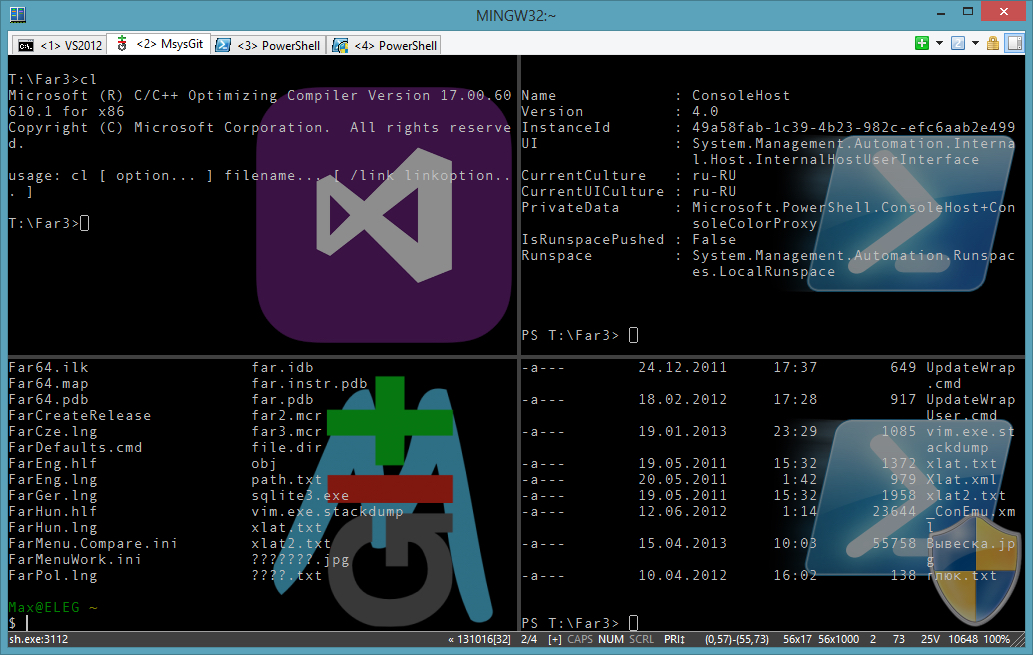
\includegraphics[scale=0.3]{img/conEmuImg.jpg}
\caption{Ukážka ConEmu emulátora}
\label{fig:test}
\end{figure}
\newpage
\subsubsection{cmder}
\indent Cmder je ďalším príkladom emulátora shell terminálu. Vychádza z troch projektov ConEmu, Clink a Git pre Windows - voľiteľná súčasť. ConEmu sme si predstavili v predcházajúcej časti s jeho kladymi a zápormi. Clink, konkrétne clink-completions je v projekte využívaný na zvýšenie komfortu pri písaní skriptov, nepridáva ďalšiu shellovú funkcionalitu. 
\paragraph{Skúsenosti}
\indent ConEmu je príjemný nástroj, dokáže zjednodušíť človeku prácu obzvlášť ak je zvyknutý na programovanie v shell scripte. Nakoľko cmder používa ConEmu ako emulátor shell terminálu a je úzko určený pre Windows platformu nemožno hovoriť o multiplatformovom riešení.
\begin{figure}[!htbp]
	\centering
	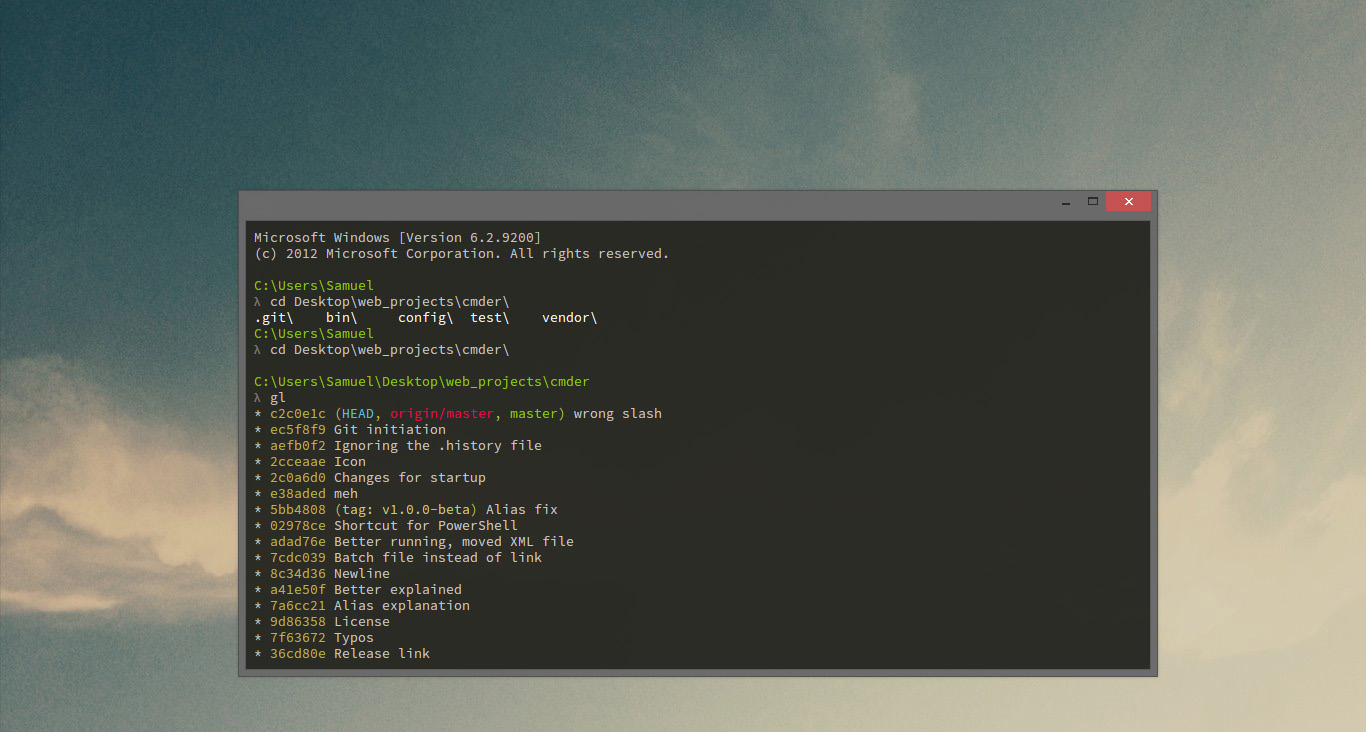
\includegraphics[scale=0.3]{img/cmder.jpg}
	\caption{Ukážka cmder emulátora}
	\label{fig:test}
\end{figure}
\newpage
\subsubsection{Babun}
\indent Babun je ďalším z množstva emulátorov pre Windows, ktorý je nadstavbou cygwinu. Vo svojom jadre používa zshell a bash, ktoré sme popísali ako populárne medzi komunitou. Prináľa vlasné gui, ktoré dokáže zafarbovať text podla zdrojoveho jazyka, čo zvyšuje prehľadnosť. Je tam git, svn, puython, perl. Tiež má integrované sťahovanie nových packagov, ktoré ponúka cygwin pomocou kľúčového slova pact. Prenositeľnosť skriptov z unixových strojov je zabezpečená tým, že používa bash a zsh, avšak je to emulátor čisto pre Windows distribúcie.
\begin{figure}[!htbp]
	\centering
	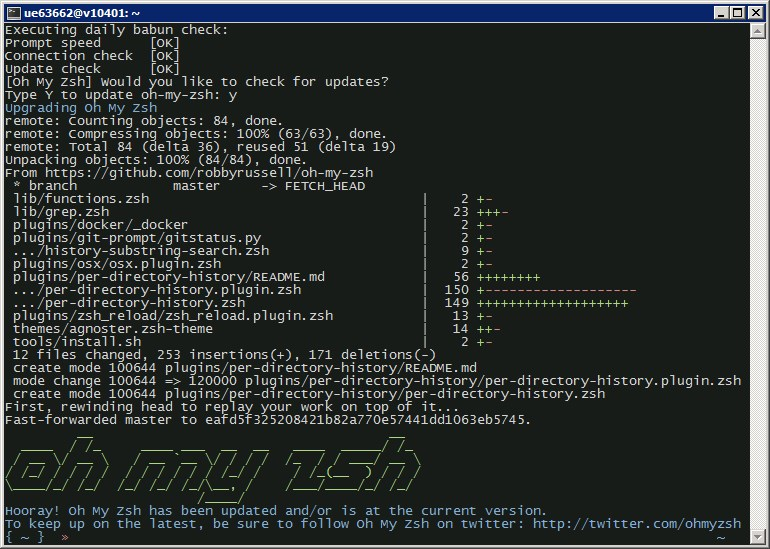
\includegraphics[scale=0.4]{img/babun.jpeg}
	\caption{Ukážka babun emulátora}
	\label{fig:test}
\end{figure}
\subsubsection{MobaXterm}
\indent Poskytuje množstvo funkcionality avšak je zatažený licenciou v hodnote 50 eur. 
\paragraph{Neplatená verzia}
\begin{itemize}
	\item Plná podpora SSH a X serveru
	\item Vzdialená plocha (RDP, VNC, Xdmcp)
	\item Vzdialený terminál (SSH, telnet, rlogin, Mosh)
	\item X11-Forwarding
	\item Automatický SFTP prehliadač
	\item Podpora pluginovt
	\item Možnosť inšalačnej alebo prenositeľnej verzie
	\item Plná dokumentácia
	\item Maximálne 12 spojení
	\item Maximálne 2 SSH tunely
	\item Maximálne 4 maká
	\item Maximálne 360 sekúnd pre Tftp, Nfs a Cron
\end{itemize}

\paragraph{Platená verzia}

\begin{itemize}
	\item Všetky vymoženosti z neplatenej verzie Home Edition +
	\item Možnosť upraviť svoju uvítaciu správu a logo
	\item Modifikovať profilový skript
	\item Odstrániť nechcené hry, šetriče obrazovky alebo nástroje
	\item Nelimitovaný počet spojení
	\item Nelimitovaný počet tunelov a makier
	\item Nelimitovaný čas behu pre sieťové daemony
	\item Podpora centrálneho hesla
	\item Profesionálny support
	\item Doživotné právo používania
\end{itemize}

\subsection{Zhodnotenie analyzovaných technológií}
\indent 

\section{Preklad jazykov}
\indent Pri programovacích jazykoch nás zaujímajú ich vyjadrovacie schopnosti ako aj vlastnosti z hľadiska ich rozpoznania. Tieto vlasnosti sa týkajú programovania a prekladu, pričom obe je potrebné zohľadniť pri tvorbe jazyka. V dnešnej dobe sa používajú na programovanie hlavne takzvané vyššie programovacie jazyky, môžeme ich označiť ako zdrojové jazyky. Na to aby vykonávali čo používateľ naprogramoval je potrebné aby boli pretransformované do jazyka daného stroja. Spomínanú transformáciu zabezpečuje prekladač, prekladačom máme na mysli program, ktorý číta zdrojový jazyk a transformuje ho do cieľového jazyka, ktorému rozumie stroj.[1]

\subsection{Kompilátor proces prekladu}
Aby bol preklad možný, musí byť zdrojový kód programu napísaný podľa určitých pravidiel, ktoré vyplývajú z jazyka. Proces prekladu je možné rodeliť na 4 hlavné časti.
\begin{itemize}
	\item lexikálna analýza
	\item syntakticka analýza
	\item spracovanie sémantiky
	\item generovanie cieľového jazyka
\end{itemize}
\indent Podrobnejšie si stručne popíšeme všetky štyri časti, ktoré majú pre nás z hľadiska prekladu najväčší zmysel.
\newline
\subsubsection{Lexikálna analýza}
	\indent Lexikálna analýza je prvou fázou kompilátora. Dopredu napísaný zdojový kód je postupne spracovávaný preprocesorom, ktorý vytvára takzvané lexémy. 
	 \newline Lexémou nazývame postupnosť alfanumerických znakov. Tieto postupnosti znakov sú následne vkladané do lexikálneho analyzátora, ktorý ma za úlohu vytvoriť zo vstupných lexém tokeny slúžiace ako vstup pre syntaktický analyzátor. 
	 \newline Tokeny sa vytvárajú na základe preddefinovaných pravidiel, ktoré sa v programovacích jazykoch definujú ako pattern. V prípade, že lexikálny analyátor nieje schopný nájsť  pattern pred danú lexému musí vyhlásiť chybu počas tokenizácie.  
	 \newline Výstupom z lexikálnej analýzy sú takzvané tokeny, ktoré tvoria vyššie jednotky jazyka ako kľúčové slová jazyka, konštanty, identifikátory, operátory a iné.
	 
	 \begin{figure}[!htbp]
	 	\centering
	 	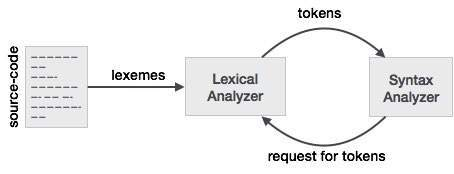
\includegraphics[width=15cm]{img/lexical_analysis.jpg}
	 	\caption{Ukážka práce lexikálneho analyzátora}
	 	\label{fig:test}
	 \end{figure}
 \newline
 
\subsubsection{Syntaktická analýza}
\indent Ďalšou fázou je syntaktická analýza. Úlohou Syntaktického analyzátora je kontrola správnosti vytvorených tokenov s uchovaním niektorých získaných informácií o štruktúre skúmanej syntaktickej jednotky. Syntaktická analýza sa radí medzi bezkontextové gramatiky. Po skoncení syntaktickej analýzy prichádza na rad sémantická analýza.

 \newline
  \newline
\begin{figure}[!htbp]
	\centering
	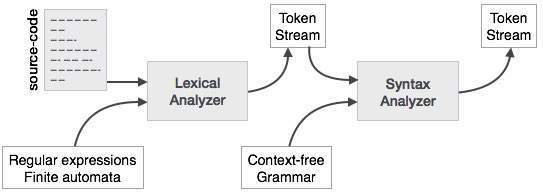
\includegraphics[width=15cm]{img/syntax_analyzer.jpg}
	\caption{Ukážka práce syntaktickeho  analyzátora}
	\label{fig:test}
\end{figure}
 \newline
 \newpage
\subsubsection{Limitácia syntaktickej analýzy}
\indent Syntaktický analyzátor ziska vstup z tokenu, ktorý vytvorí lexikálny analyzátor. Lexikálne analyzátory sú zodpovedné za validitu tokenu.Syntaktické analyzátory majú nasledovné limitácie.

\begin{itemize}
	\item nedokážu zistiť validitu tokenu
	\item nedokážu zistiť či je token používaný pred tým ako je deklarovaný
	\item nedokážu zistiť či je token používaný pred tým ako je inicializovaný
	\item nedokážu zistiť validitu operácie, ktorú token vykonáva
\end{itemize}



\subsubsection{Semantická  analýza}
\indent Sémantická analýza má za úlohu interpretovať symboly, typy, ich vzťahy.Sémantická analýza rohoduje či má syntax programy význam alebo nie.
Ako príklad zisťovania významu môžeme uviesť jednoduchú inicializáciu premennej.

\begin{lstlisting}

	int integerVariable = 6

	int secondIntegerVariable = "six"
\end{lstlisting}

Oba príklady by mali prejsť cez lexikálnu a syntaktickú analýzu. Je až na sémantickej analýze aby rozhodla o správnosti zápisu programu a v prípade nesprávneho zápisu informovala o chybe.  Hlavné úlohy sémantickej analýzy sú" :

\begin{itemize}
	\item zisťovanie dosahu definovaných tokenov takzvaný scoping
	\item kontrola typov
	\item deklaracia premenných
	\item definícia premenných
	\item viacnásobná deklarácia premenných v jedno scope
\end{itemize}

\subsubsection{Generovanie cieľového jazyka}
\indent Generovanie cieľového jazyka môžeme považovať za poslednú fázu kompilátora. V tejto fáze sa preklápa jazyk z vyššieho jazyka do strojového jazyka, ktorý úspešne prešiel cez analyzačné časti .

\subsection{Iterpreter}
\indent popis interpretera, hladam cosi schopne.

\subsection{Abeceda a vyhradené slová jazyka}
abeceda jazyka, popis ake pismena-slova rozpoznava, ake su vyhradene slova jazyka a bla bla
Doplit daco o co sa bude dat opret v navrhu a arch.

\subsection{Procedúry a algoritmy}
procedúra - konečná postupnosť inštrukcií, ktorá sa dá vykonať mechanicky. Doplit daco o co sa bude dat opret v navrhu a arch.

\section{Návrh riešenia}
\subsection{Prípady použitia}
\begin{figure}[!htbp]
	\centering
	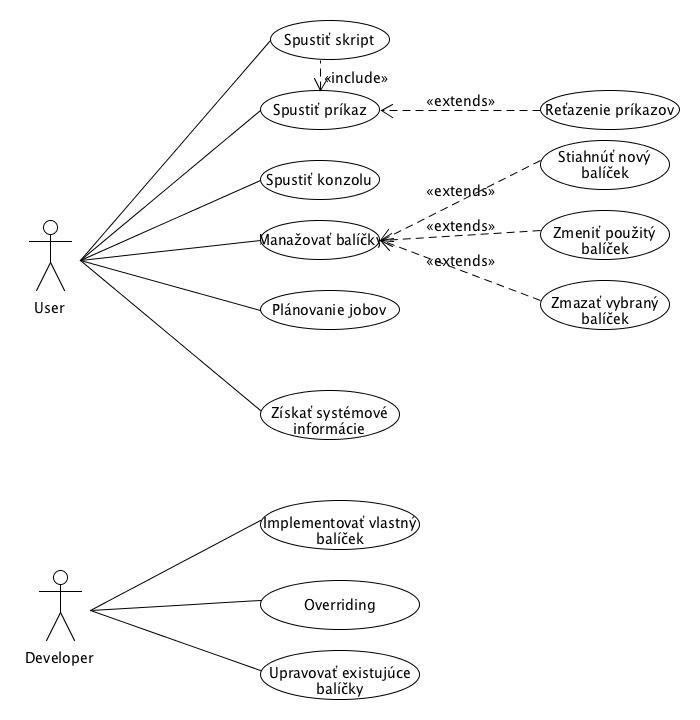
\includegraphics[scale=0.6]{img/usecase.jpg}
	\caption{Prípady použitia pre navrhovanú aplikáciu}
	\label{fig:test}
\end{figure}
\newpage
\subsection{Popis use casov}
\indent V tejto časti sa venueme popisu jednotlivých use casov. Use case diagram spolu s popisom sú základnými prvkami na ktorých je možné špecifikovať novo vznikajúci software. Je dôležité aby najpodstatnejšie časti systému boli špecifikované na začiatku, aby sa pri navrhovaní aplikácie mohli prijať rozhodnutia, ktorými bude možné zaručiť, že výsledné riešenie bude to najlepšie možné, vyhovujúce špecifikácii. Ako je zjavné aj z priloženého diagramu prípadov použitia, pre aplikáciu sme identifikovali dvoch hráčov : Vývojár skriptov a Vývojár balíčkov. Títo hráči majú jednu spoločnú črtu - pre obe platí, že hráč je vývojár. Avšak je rozdiel medzi vývojárom skriptu a vývojom nových súčastí systému, čo je zjavne vidieť aj z popisu konkrétnych prípadov použitia.
\subsubsection{Vývojár skriptov}
\indent Rola sa zameriava hlavne na používanie hotovej aplikácie, prácu s balíčkami, vytváranie skriptov, efektívne využívanie dostupného \gls{api}. 
\paragraph{Spustiť konzolu}
\begin{center}
	\begin{table}[htbp]
		\begin{tabular}{|p{2.5cm}|p{14cm}|}
			\hline
			\textbf{Use case} & Spustiť konzolu \\ 
			\hline
			\textbf{Podmienky} & Používateľ musí disponovať stiahnutou aplikáciou.\\
			\hline
			\textbf{Vstup} & Nie je potrebný žiany vstup od používateľa.\\
			\hline
			\textbf{Popis} & Konzolové rozhranie sa spustí. \\ 
			\hline
			\textbf{Výstp} & Konzola zobrazí základné údaje o konfigurácii.\\
			\hline
			\textbf{Chyba} & Konzola sa nespustí, musí však poskytnúť informáciu o chybe ktorá pri štarte nastala.\\
			\hline
		\end{tabular}
	\caption{Use case : Spustiť konzolu}
	\label{table:1}
	\end{table}
\end{center}
\newpage
\paragraph{Spustiť príkaz}
\begin{center}
	\begin{table}[htbp]
		\begin{tabular}{|p{2.5cm}|p{14cm}|}
		\hline
		\textbf{Use case} & Spustiť príkaz \\ 
		\hline
		\textbf{Podmienky} & Shell aplikácia musí byť spustená \\ 
		\hline
		\textbf{Vstup} & Textový reťazec obsahujúci príkaz a jeho argumenty.\\
		\hline
		\textbf{Popis} & Používateľ zadá valídny príkaz, následne získa výstup pre zadaný príkaz. \\ 
		\hline
		\textbf{Výstp} & Textový reťazec, ktorý v závislosti od programu variuje v dľžke a obsahu.\\
		\hline
		\textbf{Chyba} & V prípade zlyhania je používateľ informovaný o probléme, ktorý nastal.\\
		\hline
		\end{tabular}
	\caption{Use case : Spustiť príkaz}
	\label{table:1}
	\end{table}
\end{center}
\paragraph{Spustiť skript}
\begin{center}
	\begin{table}[htbp]
		\begin{tabular}{|p{2.5cm}|p{14cm}|}
			\hline
			\textbf{Use case} & Spustiť skript \\ 
			\hline
			\textbf{Podmienky} & Shell aplikácia musí byť spustená a skript správne napísaný.\\ 
			\hline
			\textbf{Vstup} & Vstupom je skript, ktorý v hlavičke definuje balíčky ktoré bude používať. Za nimi môže nasledovať čokoľvek od definície premenných, funkcií. V tele skriptu musí byť zadefinovaná metóda main(String args).\\
			\hline
			\textbf{Popis} & Vykonajú sa všetky príkazy tak ako sú napísané v zdrojovom súbore. \\ 
			\hline
			\textbf{Výstp} & Výstup je textový reťazec, závislý na logike skriptu.\\
			\hline
			\textbf{Chyba} & V prípade chyby pri sťahovaní závislostí, exekúcie príkazov, alebo iných komplikácií za behu program zapisuje na stderr chybové hlášky spolu zo základným popisom problému, tracom.\\
			\hline
		\end{tabular}
	\label{table:1}
	\caption{Use case : Spustiť skript}
	\end{table}
\end{center}
\newpage
\paragraph{Spustiť shell príkaz}
\begin{center}
	\begin{table}[htbp]
		\begin{tabular}{|p{2.5cm}|p{14cm}|}
			\hline
			\textbf{Use case} & Spustiť shell príkaz \\ 
			\hline
			\textbf{Podmienky} & Shell aplikácia musí byť spustená a skript správne napísaný. Taktiež musí byť v operačnom systéme ktorý podporuje shell. \\ 
			\hline
			\textbf{Vstup} & Textový reťazec obsahujúci príkaz a jeho argumenty.\\
			\hline
			\textbf{Popis} & Používateľ zadá valídny príkaz, následne získa výstup pre zadaný príkaz. \\ 
			\hline
			\textbf{Výstp} &Textový reťazec, ktorý v závislosti od programu variuje v dľžke a obsahu. \\
			\hline
			\textbf{Chyba} & V prípade zlyhania je používateľovi vratený chybový kód.\\
			\hline
		\end{tabular}
	\label{table:1}
	\caption{Use case : Spustiť shell príkaz}
	\end{table}
\end{center}
\paragraph{Spustiť powershell príkaz}
\begin{center}
	\begin{table}[htbp]
		\begin{tabular}{|p{2.5cm}|p{14cm}|}
			\hline
			\textbf{Use case} & Spustiť powershell príkaz \\ 
			\hline
			\textbf{Podmienky} & Shell aplikácia musí byť spustená a skript správne napísaný. Systém musí mať nainštalovaný powershell.\\ 
			\hline
			\textbf{Vstup} & Textový reťazec obsahujúci príkaz a jeho argumenty.\\
			\hline
			\textbf{Popis} & Používateľ zadá valídny príkaz, následne získa výstup pre zadaný príkaz. \\ 
			\hline
			\textbf{Výstp} &Textový reťazec, ktorý v závislosti od programu variuje v dľžke a obsahu. \\
			\hline
			\textbf{Chyba} & V prípade zlyhania je používateľovi vratený chybový výstup z powershellu.\\
			\hline
		\end{tabular}
	\label{table:1}
	\caption{Use case : Spustiť powershell príkaz}
	\end{table}
\end{center}
\newpage
\paragraph{Reťazie príkazov}
\begin{center}
	\begin{table}[htbp]
		\begin{tabular}{|p{2.5cm}|p{14cm}|}
			\hline
			\textbf{Use case} & Reťazie príkazov \\ 
			\hline
			\textbf{Podmienky} & Shell aplikácia musí byť spustená. Vstup musí byť zadaný v správnom formáte.\\ 
			\hline
			\textbf{Vstup} & Textový reťazec obsahujúci sekvenciu príkazov, ich argumenty spojené znakom pajpy "|".\\
			\hline
			\textbf{Popis} & Systém rozozná, že ide o zreťazený príkaz a následne začne vykonávať príkazy v poradí v akom boli zadané. Jednotlivé príkazy odovzdajú svoje výstupy svojmu nasledovníkovy po úspešnom ukončení. Príkazy sa vykonávajú až kým nepríde na posledný príkaz v sekvencii, alebo ako počas behu príde pri niektorom z príkazov ku chybe. O chybe je používateľ oboznámený a chyba je zapísaná na štandardný chybový výstup. \\ 
			\hline
			\textbf{Výstp} & Textový reťazec, ktorý v závislosti od programu variuje v dľžke a obsahu, výstup bude vygenerovaný posledným príkazom sekvencie.\\
			\hline
			\textbf{Chyba} & O chybe je používateľ oboznámený a chyba je zapísaná na štandardný chybový výstup.\\
			\hline
		\end{tabular}
	\label{table:1}
	\caption{Use case : Reťazie príkazov}
	\end{table}
\end{center}


\paragraph{Manažovať balíčky}
\begin{center}
	\begin{table}[htbp]
		\begin{tabular}{|p{2.5cm}|p{14cm}|}
			\hline
			\textbf{Use case} & Manažovať balíčky \\ 
			\hline
			\textbf{Podmienky} & Shell aplikácia musí byť spustená.\\ 
			\hline
			\textbf{Vstup} & Textový reťazec obsahujúci príkaz "pkg" alebo aky si vyberem a jeho argumenty.\\
			\hline
			\textbf{Popis} & Používateľ bude schopný nahrať, zmazať, nahradiť vybraný balíček. \\ 
			\hline
			\textbf{Výstp} & Textový reťazec, ktorý v závislosti od programu variuje v dľžke a obsahu - možno bude informovať o šťahovacom procese.\\
			\hline
			\textbf{Chyba} & O chybe je používateľ oboznámený a chyba je zapísaná na štandardný chybový výstup v podobe stack tracu napr. .\\
			\hline
		\end{tabular}
	\label{table:1}
	\caption{Use case : Manažovať balíčky}
	\end{table}
\end{center}
\newpage
\paragraph{Stiahnúť nový balíček}
\begin{center}
	\begin{table}[htbp]
		\begin{tabular}{|p{2.5cm}|p{14cm}|}
			\hline
			\textbf{Use case} & Stiahnúť nový balíček \\ 
			\hline
			\textbf{Podmienky} & Shell aplikácia musí byť spustená. Príkaz na stiahnutie balíčka musí byť správne zadaný.\\ 
			\hline
			\textbf{Vstup} & Textový reťazec obsahujúci príkaz "pkg download <názov balička>"\\
			\hline
			\textbf{Popis} & Program sa ako prvé pozrie do adresára balíčkov či už daný balíček nebol stiahnutý, ak nie stiahne nový balíček a načíta ho medzi aktívne balíčky. V opačnom prípade medzi aktívne balíčky načíta používateľom zvolený balíček.\\ 
			\hline
			\textbf{Výstp} & Textový reťazec  informujúci o úspešnosti sťahovania.\\
			\hline
			\textbf{Chyba} & Vypíše chybu do stderr v prípade, že daný balíček na servery neexistuje, používateľ nemá internetové pripojenie.\\
			\hline
		\end{tabular}
		\label{table:1}
		\caption{Use case : Stiahnúť nový balíček}
	\end{table}
\end{center}
\paragraph{Zmeniť  použiťý balíček}
\begin{center}
	\begin{table}[htbp]
		\begin{tabular}{|p{2.5cm}|p{14cm}|}
			\hline
			\textbf{Use case} & Zmeniť  použiťý balíček \\ 
			\hline
			\textbf{Podmienky} & Shell aplikácia musí byť spustená. Príkaz na zmenenie používaného balíčka musí byť správne zadaný.\\ 
			\hline
			\textbf{Vstup} & Textový reťazec obsahujúci príkaz "pkg change <názov nahradzovaného balička> <názov nahradzujúceho balička>\\
			\hline
			\textbf{Popis} & Program zmení používaný balíček z aktuálne používaného na balíček vybratý používateľom. Táto voľba je aplikovateľná iba pre spravovanie verzií existujúcich balíčkov. V prípade, že nahradzujúci balíček nieje dostupný lokálne, používateľ bude vyzvaný stiahnúť daný balíček.\\ 
			\hline
			\textbf{Výstp} & Textový reťazec informujúci o úspešnosti výmeny, alebo informujúci o potrebe stiahnutia balíčka.\\
			\hline
			\textbf{Chyba} & V prípade ak príde počas zmeny balíčkov k chybe, bude zapísana na stderr.\\
			\hline
		\end{tabular}
		\label{table:1}
		\caption{Use case : Zmeniť  použiťý balíček}
	\end{table}
\end{center}
\newpage
\paragraph{Zmazať vybraný balíček}
\begin{center}
	\begin{table}[htbp]
		\begin{tabular}{|p{2.5cm}|p{14cm}|}
			\hline
			\textbf{Use case} & Zmazať vybraný balíček \\ 
			\hline
			\textbf{Vstup} & Textový reťazec obsahujúci príkaz "pkg delete <názov balička>.\\
			\hline
			\textbf{Podmienky} & Shell aplikácia musí byť spustená. Príkaz na zmazanie vybraného balíčka musí byť správne zadaný.\\ 
			\hline
			\textbf{Popis} & Program zmaže používateľom vybraný balíček z aktívnych balíčkov a následne ho fyzicky zmaže z disku. \\
			\hline
			\textbf{Výstp} & Textový reťazec informujúci o úspešnosti zmazania zadaného balíka\\
			\hline
			\textbf{Chyba} & V prípade nesprávneho odstránenia balíčka z aktívnych alebo pri následnom mazaní zo súborového systému bude informácia o chybe presmerovaná na stderr.\\
			\hline
		\end{tabular}
		\label{table:1}
		\caption{Use case : Zmazať vybraný balíček}
	\end{table}
\end{center}
\paragraph{Získať systémové informácie}
\begin{center}
	\begin{table}[htbp]
		\begin{tabular}{|p{2.5cm}|p{14cm}|}
			\hline
			\textbf{Use case} & Získať systémové informácie \\ 
			\hline
			\textbf{Vstup} & Vstupom je textový reťazec "sysinfo".\\
			\hline
			\textbf{Podmienky} & Shell aplikácia musí byť spustená. Používateľ vloží valídny príkaz na vyžiadanie systémových informácií. \\ 
			\hline
			\textbf{Popis} & Program vypíše na štandardný výstup informácie o systémových informáciách ako napríklad využitie procesoru, využitie pamäte RAM, využitie oddielu swap, teplotu zariadení a podobné.\\ 
			\hline
					
			\textbf{Výstp} & Výstupom je textový reťazec, formátovaný do riadkov. Každému riadku prislúcha jedna informácia napr. CPU, ďalší riadok RAM atď.. V prípade viac jadrového procesora sa vypísu informácie o každom z jadier.  \\
			\hline
		\end{tabular}
	\end{table}
\newpage
\begin{table}[htbp]
\begin{tabular}{|p{2.5cm}|p{14cm}|}
\hline
			\textbf{Chyba} & V prípade, že používateľ nemá právo na získanie informácií program vypíse dôvod priamo na stdout. Tak isto tam vypíše aj akékoľvek chyby ku ktorým môže prísť počas behu.\\
			\hline
		\end{tabular}
		\label{table:1}
		\caption{Use case : Získať systémové informácie}
	\end{table}
\end{center}

\paragraph{Získať informácie o procesoch}
\begin{center}
	\begin{table}[htbp]
		\begin{tabular}{|p{2.5cm}|p{14cm}|}
			\hline
			\textbf{Use case} & Získať informácie o procesoch \\ 
			\hline
			\textbf{Vstup} & Vstupom je textový reťazec "processes".\\
			\hline
			\textbf{Podmienky} & Shell aplikácia musí byť spustená. Používateľ vloží valídny príkaz na vyžiadanie informácií o procesoch. \\ 
			\hline
			\textbf{Popis} & Program vypíše na štandardný výstup informácie o bežiacich procesoch, používateľoch, ktorý tieto procesy spúšťajú, koľko procesoru, pamäte RAM pouýívajú.\\ 
			\hline
			\textbf{Výstp} & Výstupom je prehľadný výpis v podobe tabuľky, kde každý riadok zodpovedá jednému procesu. Nad jednotlivými hodnotami je hlavný riadok, ktorý popisuje o akú hodnotu ide.\\
			\hline
			\textbf{Chyba} & V prípade, že nieje možné získať informácie o procesoch je táto skutočnosť zobrazená na stdout a popis chyby sa presmeruje na stderr.\\
			\hline
		\end{tabular}
		\label{table:1}
		\caption{Use case : Získať informácie o procesoch}
	\end{table}
\end{center}
\newpage
\paragraph{Presmerovať chybový výstup}
\begin{center}
	\begin{table}[htbp]
		\begin{tabular}{|p{2.5cm}|p{14cm}|}
			\hline
			\textbf{Use case} & Presmerovať chybový výstup \\ 
			\hline
			\textbf{Vstup} & Pre presmerovanie na chybový výstup je potrebné dodržať syntax command stderr> file\\
			\hline
			\textbf{Podmienky} & Shell aplikácia musí byť spustená. Používateľ vloží valídny príkaz na presmerovanie chybového výstupu. \\ 
			\hline
			\textbf{Popis} & Program presmeruje chybový výstup kam mu používateľ v príkaze prikáže. \\ 
			\hline
			\textbf{Výstp} & Výstup programu predstavuje textový reťazec s popisom chyby, ktorá nastala.\\
			\hline
			\textbf{Chyba} & Ak by došlo k chybe zaloguje sa do logu aplikácie.\\
			\hline
		\end{tabular}
		\label{table:1}
		\caption{Use case : Presmerovať chybový výstup}
	\end{table}
\end{center}
\paragraph{Presmerovať štandardný výstup}
\begin{center}
	\begin{table}[htbp]
		\begin{tabular}{|p{2.5cm}|p{14cm}|}
			\hline
			\textbf{Use case} & Presmerovať štandardný výstup \\ 
			\hline
			\textbf{Podmienky} & Shell aplikácia musí byť spustená. Používateľ vloží valídny príkaz na presmerovanie štandardného výstupu. \\ 
			\hline
			\textbf{Vstup} & Pre presmerovanie na štandardný výstup je potrebné dodržať syntax command stderr> file\\
			\hline
			\textbf{Popis} & Program presmeruje štandardný výstup kam mu používateľ v príkaze prikáže.\\ 
			\hline
			\textbf{Výstp} & Výstup programu predstavuje textový reťazec s výstupom zo skriptu alebo príkazu.\\
			\hline
			\textbf{Chyba} & Ak by došlo k chybe zaloguje sa do logu aplikácie.\\
			\hline
		\end{tabular}
		\label{table:1}
		\caption{Use case : Presmerovať štandardný výstup }
	\end{table}
\end{center}
\newpage
\paragraph{Vynútiť ukončenie procesu}
\begin{center}
	\begin{table}[htbp]
		\begin{tabular}{|p{2.5cm}|p{14cm}|}
			\hline
			\textbf{Use case} & Vynútiť ukončenie procesu \\ 
			\hline
			\textbf{Vstup} & Pre vynútenie ukončenia procesu je potrebné použitie kľúčového slova kill <pid>.\\
			\hline
			\textbf{Podmienky} & Shell aplikácia musí byť spustená. Používateľ vloží valídny príkaz na ukončenie procesu. \\ 
			\hline
			\textbf{Popis} & Program presmeruje štandardný výstup kam mu používateľ v príkaze prikáže.\\ 
			\hline
			\textbf{Výstp} & Výstup programu je textový reťazec informujúci o úspešnosti ukončenia procesu.\\
			\hline
			\textbf{Chyba} & Ak pri ukončovaní procesu príde k chybe, informácie sa presunú na stderr.\\
			\hline
		\end{tabular}
		\label{table:1}
		\caption{Use case : Vynútiť ukončenie procesu}
	\end{table}
\end{center}

\paragraph{Vytvoriť funkciu}
\begin{center}
	\begin{table}[htbp]
		\begin{tabular}{|p{2.5cm}|p{14cm}|}
			\hline
			\textbf{Use case} & Vytvoriť funkciu \\ 
			\hline
			\textbf{Podmienky} & Používateľ musí mať prístup k akémukoľvek textovému editoru.  \\ 
			\hline
			\textbf{Vstup} & Funkcia musí byť správne zadefinovaná. 
			Synax pre definovanie funkcie : 
			function <návratový typ> <názov funkcie>(parametre funkcie){telo funkcie}. \\
			\hline
			\textbf{Popis} & Používateľ napíše funkciu, ktorá bude prečítaná programom a vykonaná.\\ 
			\hline
			\textbf{Výstp} & Funkcia vracia premennú s definovanou návratovou hodnotou.\\
			\hline
			\textbf{Chyba} & V prípade, že nastane chyba pri exekúcii funkcie program skončí a program zapíše informácie o chybe na stderr.\\
			\hline
		\end{tabular}
		\label{table:1}
		\caption{Use case : Vytvoriť funkciu}
	\end{table}
\end{center}
\newpage
\paragraph{Override funkcie}
\begin{center}
	\begin{table}[htbp]
		\begin{tabular}{|p{2.5cm}|p{14cm}|}
			\hline
			\textbf{Use case} & Override funkcie \\ 
			\hline
			\textbf{Podmienky} & Používateľ musí mať prístup k akémukoľvek textovému editoru.  \\ 
			\hline
			\textbf{Vstup} & Nad funciou je potrebné zapísať @Override alebo @Override(číslo) čo prekladaču povie, že má používať práve túto verziu funkcie, v druhom prípade číslo značí prioritu pri prepisovaní. Najnižšia priorita je 1, metóda s najvžšším číslom teda s najvyššou prioritou bude použitá v skripte.\\
			\hline
			\textbf{Popis} & Používateľ napíše funkciu, ktorá bude prečítaná programom a vykonaná. Navyše bude nahradzovať funkciu s rovnakým názvom.\\ 
			\hline
			\textbf{Výstp} & Premenná, ktorá je uvedená v definícii funkcie.\\
			\hline
			\textbf{Chyba} & V prípade zle zadefinovanej syntaxe je problém zapísaný na stderr a vykonávanie skriptu je ukončené.\\
			\hline
		\end{tabular}
		\label{table:1}
		\caption{Use case : Override funkcie}
	\end{table}
\end{center}
\subsubsection{Vývojár balíčkov}
\indent Ako je z názvu role zjavné, tento hráč bude mať na starosti hlavne vývoj aplikácie, starať sa o jej funkcionalitim v zmysle rozširovania API, ktoré môže vývojár skriptov používať pre efektívnejšiu prácu.
\paragraph{Implementovať vlastný balíček}
\begin{center}
	\begin{table}[htbp]
		\begin{tabular}{|p{2.5cm}|p{14cm}|}
			\hline
			\textbf{Use case} & Implementovať vlastný balíček \\ 
			\hline
			\textbf{Podmienky} & Používateľ musí mať nainštalovanú Java SDK vo verzii 8, mať prístup k textovému editoru.  \\ 
			\hline
			\textbf{Vstup} & Balíček obsahujúci všetky potrebné rozhrania, ktoré musí vývojár balíčka implementovať.\\
			\hline
			\textbf{Popis} & Používateľ implementuje novú funkcionalitu v jave, následne všetky zdrojové súbory skompiluje a pridá do jar súboru určeného na ukladanie nových balíčkov.\\ 
			\hline
			\textbf{Výstp} & Balíček, ktorý je možné nahrať do aplikácie a používať ako jeden z príkazov.\\
			\hline
			\textbf{Chyba} & Chyba môže nastať pri vytváraní balíčka, kedy ho o chybe informuje prekladač jazyka v ktorom je balíček implementovaný. V prípade neúspešného načítania je používateľ informovaný priamo v konzole na stout.\\
			\hline
		\end{tabular}
		\label{table:1}
		\caption{Use case : Implementovať vlastný balíček}
	\end{table}
\end{center}
\newpage
\paragraph{Upravovať existujúce balíčky}
\begin{center}
	\begin{table}[htbp]
		\begin{tabular}{|p{2.5cm}|p{14cm}|}
			\hline
			\textbf{Use case} & Upravovať existujúce balíčky \\ 
			\hline
			\textbf{Podmienky} &  Používateľ musí mať nainštalovanú Java SDK vo verzii 8, mať prístup k textovému editoru.  \\ 
			\hline
			\textbf{Vstup} & Zdrojové súbory už existujúceho balíčka.\\
			\hline
			\textbf{Popis} & Používateľ upraví implementáciu alebo pridá novú funkcionalitu v jave, následne všetky zdrojové súbory skompiluje a pridá do jar súboru určeného na ukladanie nových balíčkov\\ 
			\hline
			\textbf{Výstp} & Po úprave je balíček možné nahrať do aplikácie a používať ako jeden z príkazov.\\
			\hline
			\textbf{Chyba} & \\
			\hline
		\end{tabular}
		\label{table:1}
		\caption{Use case : Upravovať existujúce balíčky}
	\end{table}
\end{center}

\subsection{Prvotný nástrel}
\subsection{Oddelenie štruktúry}

\section{Architektúra aplikácie}
\indent Ako sme ukázali existuje veľké množstvo skiptovacích jazykov ci, ktoré dokážu efektívne automatizovať dennodennú prácu avšak majú jeden spoločný nedostatok - nie sú multiplatformové. Táto vlastnosť môže byť  pre niekoho nepodstatná, no pri veľkých projektoch kde sa míňa množstvo prostriedkov na automatizáciu to až tak zanedbateľný fakt nie je. Stačí si len predstaviť koľko času zabere tvorba automatizovaných skriptov pre jednu platformu a pripočítať rovnaké množstvo času pre každú ďalšiu. Niekto by mohol namietať, že pre ďalšie platformy to toľko času nezabere nakoľko logika skriptov je uz definovaná. Tu treba brať ohľad na to, že nie každý jazyk poskytuje programátorovi rovnaké API a teda treba rátať s možnosťou, že niekde bude potrebné doimplementovať veci chýbajúce v jazyku. Preto vyššie spomenuté dôvody sme sa rozhodli pre vytvorenie nového jazyka, ktorý by bol jednoducho rozšíriteľný, manažovateľný, ľahko pisateľný a platformovo nezávislý. \cite{morf}

\subsection{Java}
\indent Je vyvíjaný spoločnosťou Oracle. Jeho syntax vychádza z jazykov C a C++. Zdrojové programy sa nekompilujú do strojového kódu, ale do medzistupňa, tzv. „byte-code“, ktorý nie je závislý od konkrétnej platformy. Táto vlastnosť Javy nám veľmi vyhovuje pre dosiahnutie cieľa platformovej nezávislosti. Ďalším veľmi podstatným faktom je, že v Jave programuje veľké množstvo developerov, tým pádom majú open source projekty veľkú šancu, že si ich komunita devoloperov osvojí a prispeje k ich postupnému zlepšovaniu.

\subsection{Pouzite navrhove vzory}
Aby sme zaručili rozšíriteľnosť, manažovateľnosť a ďalšie zásady dobrého softwéru bolo potrebné zvoliť vhodnú arhitektúru, ktorú popisujú použité návrhové vzory.
\subsubsection{Command - príkaz}
\indent Command pattern je známy behaviorálny návrhový vzor, používa sa najmä na menežovanie algoritmov, vzťahov a zodpovednosti medzi objektami. 
Cieľom vzoru je zapúzdriť požiadavku(request) ako objekt tým pádom parametrizovať klienta s rôznymi požiadavkami a zabezpečiť operáciu spať.
\begin{figure}[!htbp]
	\centering
	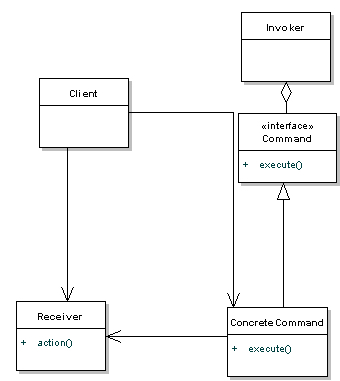
\includegraphics[width=10cm]{img/command_pattern_class.jpg}
	\caption{Class diagram Command návrhového vzoru}
	\label{fig:test}
\end{figure}
\newline
Command vzor deklaruje rozhranie pre všetky budúce commandy a zároveň execute() metódu, ktorú s vypýta Receiver commandu aby splnil požadovanú operáciu.
Receiver je objekt, ktorý vie ako požadovanú operáciu splniť. Invoker pozná command a pomocou implementovanej execute() metódy dokáže vyvolať požadovanú operáciu.
Klient potrebuje implemenotvaž ConcreteCommand a nastavit Receiver pre command. ConcreteCommand definuje spojenie medzi action a receiver. Keď Invoker zavolá execute() metódu na ConcreteCommand spustí tým jednu alebo viac akcií, ktoré budú bežať pomocou Receivera.

Pre lepšie pochopenie je proces zobrazený aj na sekvenčnom diagrame.
\begin{figure}[!htbp]
	\centering
	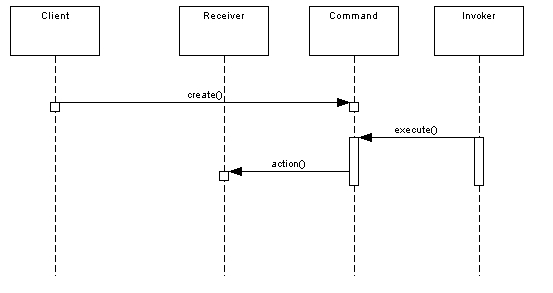
\includegraphics[width=10cm]{img/command_seq.jpg}
	\caption{Sekvenčný diagram Command návrhového vzoru}
	\label{fig:test}
\end{figure}
\newline

\subsubsection{Factory - továreň}
\indent Factory návrhový vzor patrí do sekcie vytváracích vzorov, pomocou tohoto vzoru budeme schopný vytvárať objekty bez toho aby sme prezradili logiku ich vytvárania klientovi.
Diagram návrhového vzoru je mozné vidieť na nasledujúcom obrázku.
\begin{figure}[!htbp]
	\centering
	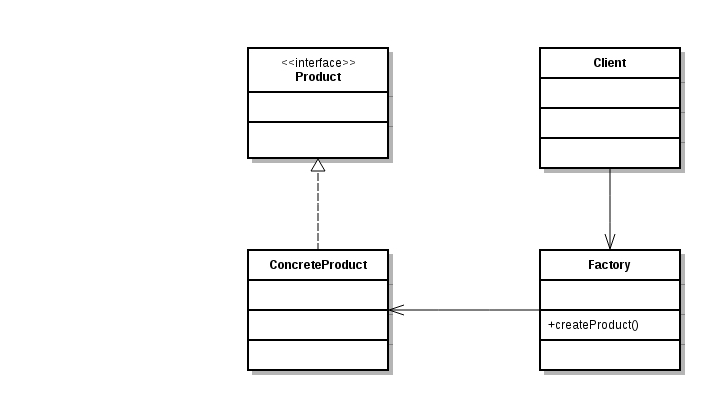
\includegraphics[width=10cm]{img/factory_design_pattern.jpg}
	\caption{Class diagram Factory návrhového vzoru}
	\label{fig:test}
\end{figure}
\newline

\subsubsection{Interpreter}
mozno pouzijem
\subsection{Komponenty aplikácie}
\indent Ako prvé bolo treba zistiť z akých komponentov sa bude aplikácia skladať. Bolo treba zamyslieť sa čo a ako to chceme dosiahnuť. v prvom návrhu sme identifikovali nasledovné komponenty. Rozhodli sme sa, že vytvoríme plugin systém kvôli tomu, čo najdem a napíšem do analyzy.
\begin{itemize}
	\item Parser - vstupov aj vystupov
	\item Loader jar súborov
	\item Sťahovač dependencií - jarka ktoré momentálne produkt neobsahuje napr. cusotm riešenia
	\item Scoping
\end{itemize}

 \begin{figure}[!htbp]
	\centering
	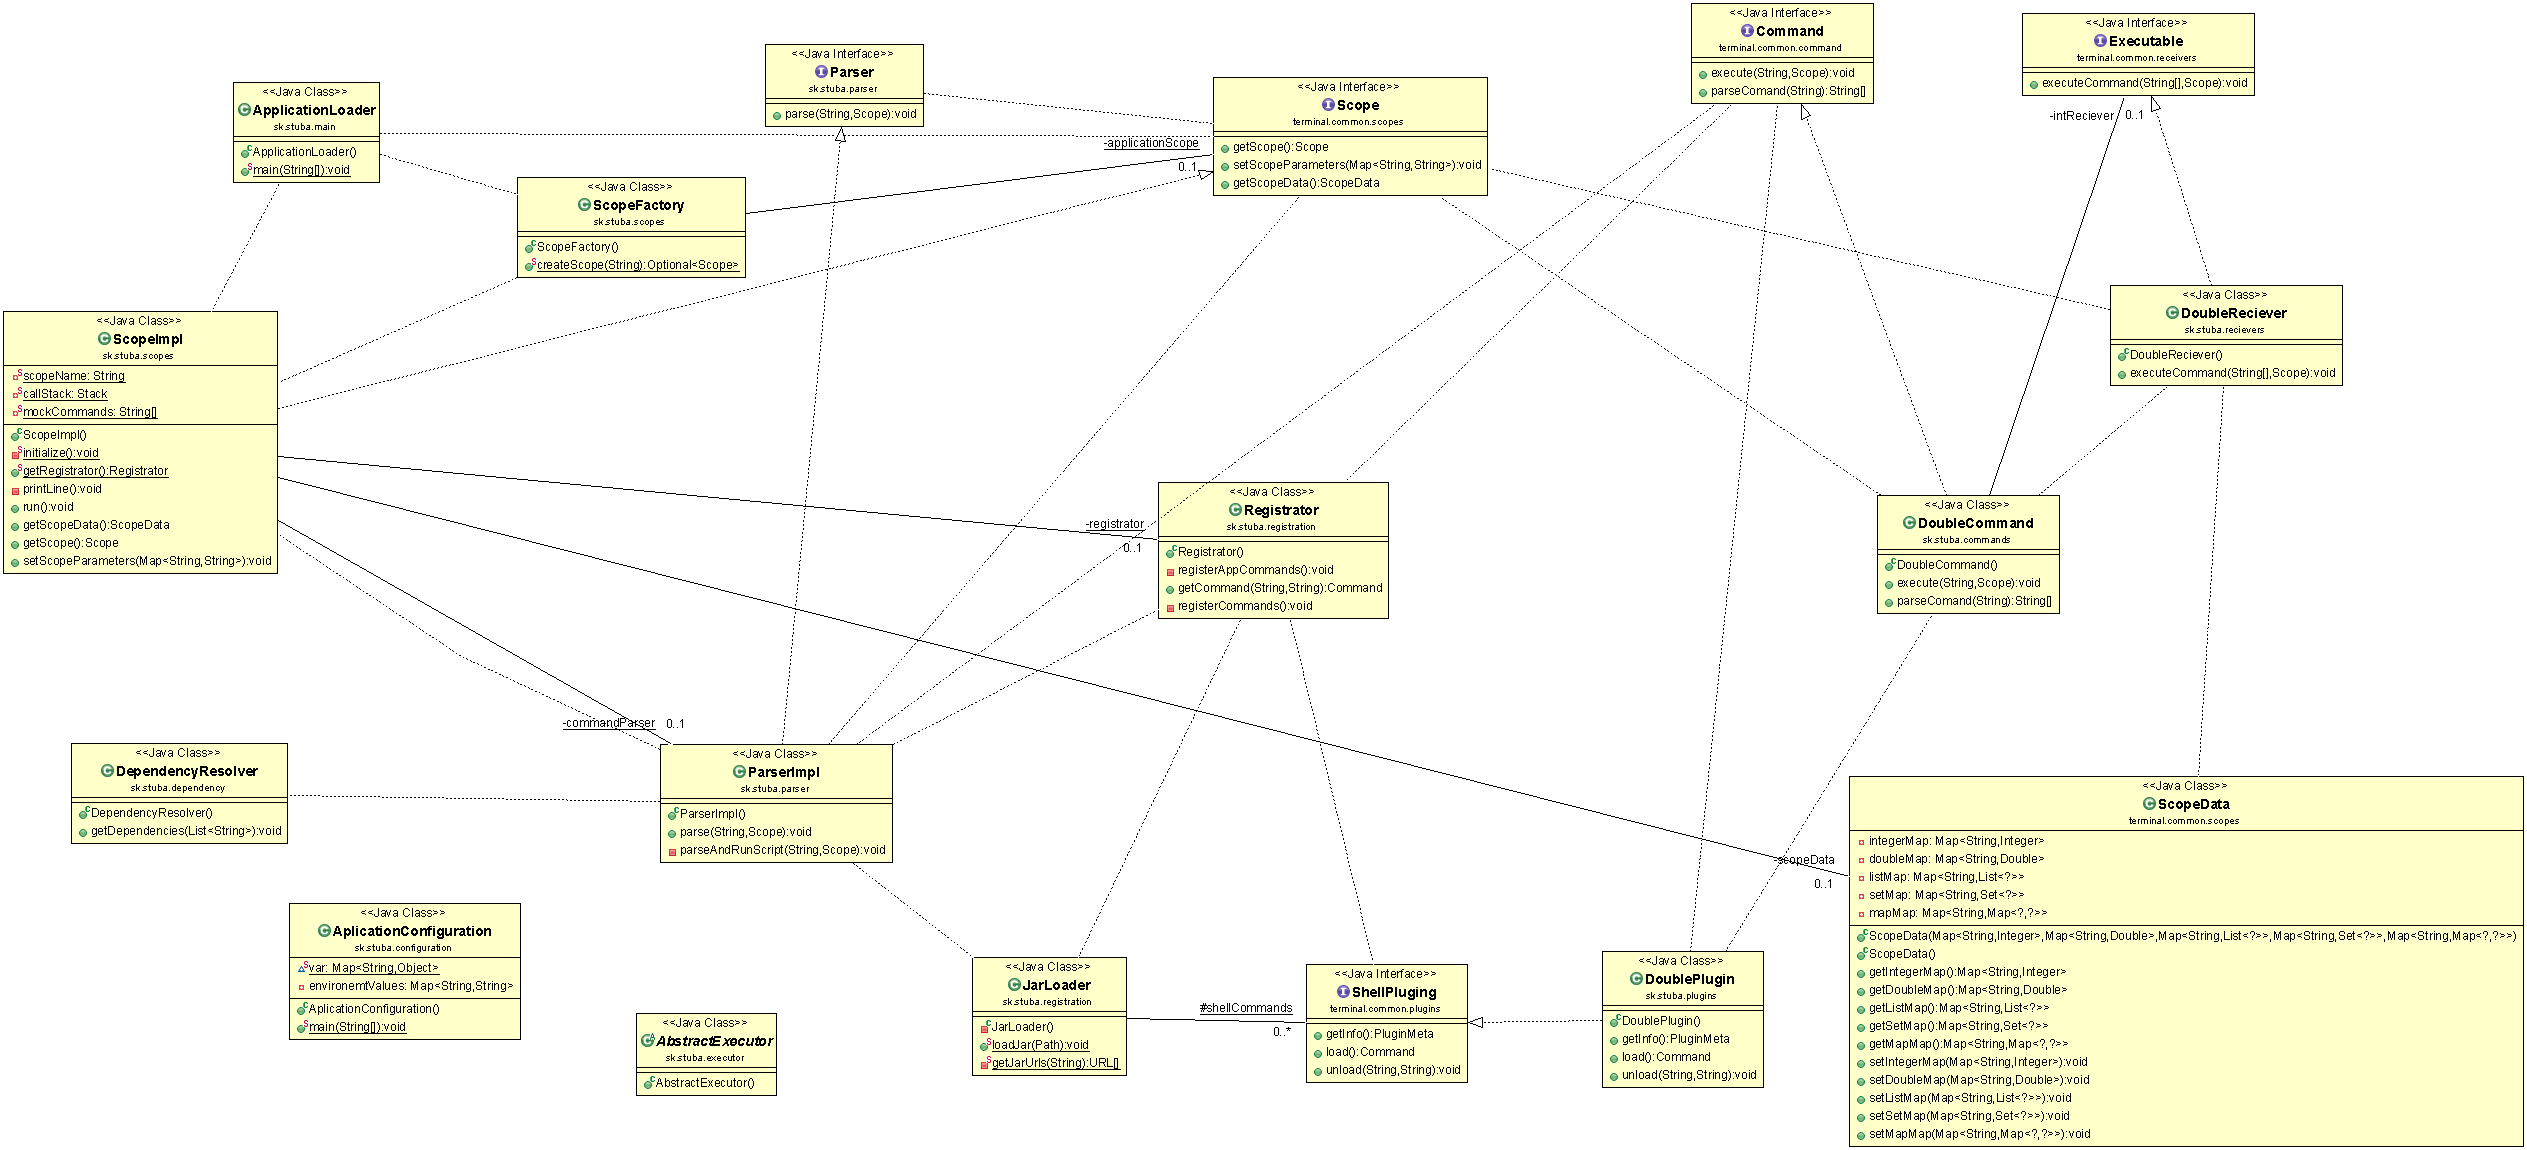
\includegraphics[width=15cm]{img/first_attemp_class_diag.jpg}
	\caption{Pvrvé funkčné riešenie}
	\label{fig:test}
\end{figure}
\newline
Z nasledovného class diagramu nebolo na prvý pohľad zreteľne viditeľné aké komponenty v programe existujú preto bolo potrebné zamyslieť sa ako by sa dali tieto časti rozumne rodeliť. Z prvotného návrhu sme vytiahli plugin. Pre implementáciu pluginu sme sa rozhodli použiť architektúru command patternu. Class diagram implementácie je viditeľný na nasledovnom obrázku.
 \begin{figure}[!htbp]
	\centering
	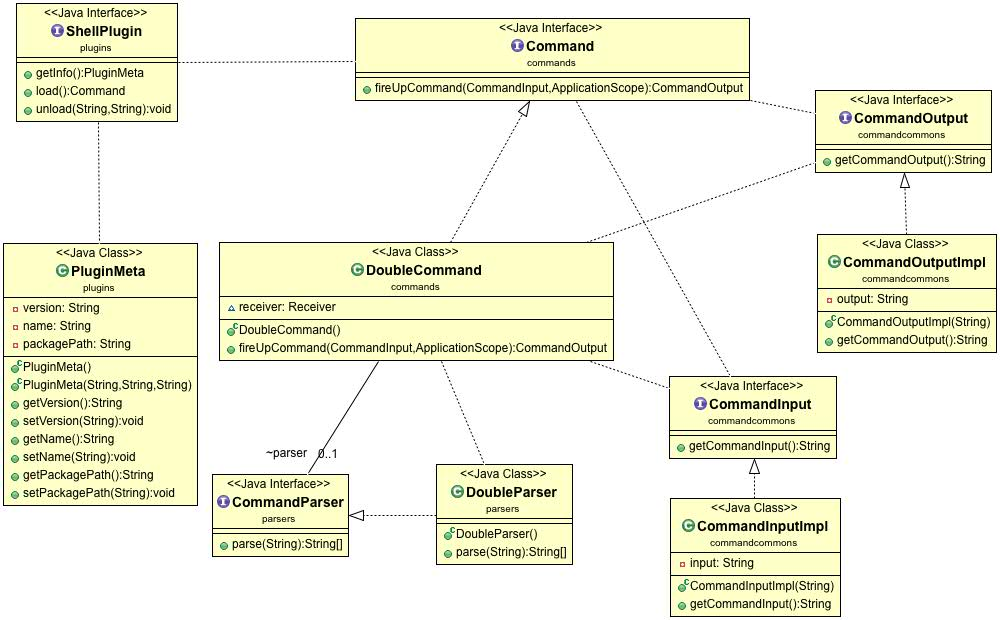
\includegraphics[width=15cm]{img/plugin_class.jpg}
	\caption{Class diagram pluginu}
	\label{fig:test}
\end{figure}
\newline
Popisat scoping
Vytvaranie commandov

\section{Zhodnotenie výsledkov}
Zatiaľ sa toho nespravilo hodne ale verím, že sa to tu cele zaplní.